\documentclass{article}

\usepackage[utf8]{inputenc}
\usepackage{url}
\usepackage{hyperref}
\usepackage{graphicx}
\usepackage{amsmath}

\graphicspath{{./images/}}

\title{An Uniswap Tour}
\author{Diego Ximenes Mendes}

\begin{document}

\date{}
\maketitle

A brief guide on some Uniswap protocol concepts.
This article was written, so I can revisit these concepts in the future, since Uniswap V3 white paper is not so explicit and didactic.
However I realized it can also be useful to others.
It includes some approaches and opinions that were not found in the current literature.
Target audience are people who have some familiarity on how Uniswap operates, at least on an user (liquidity provider and trader) level.

\section{Constant Product Market Maker}

In a Constant Product Market Maker, such as implemented by Uniswap V2, there are two types of actors, traders and liquidity providers.

Traders are interested to exchange a certain amount of a token for a certain amount of another token, and for that they generally pay a fee to use a service, a market maker, that enables that operation.

Liquidity providers are the ones who previously provide tokens to the market maker, to then be used by traders to execute their exchanges.
In general, fees gathered from traders are distributed to liquidity providers, which are then incentivized to provide their tokens to the market maker.

Also, Uniswap defines the concept of a pool, which is a Constant Product Market Maker specific for a pair of tokens, e.g., USDC/DAI, in which liquidity providers and traders operate with only this pair of tokens.

Each kind of those operations have its own invariances considering the state of a pool.

\subsection{Traders Operations Invariance}
\label{section:traders_invariance}

Considering a pool of a pair of tokens $token_x$ and $token_y$, and that in the current pool's state the amount of $token_x$ is $x$, and the amount of $token_y$ is $y$, and $k$ as a constant, a Constant Product Market Maker defines the following invariance for traders operations:

\begin{equation}
    \label{equation:constant_product}
    xy=k
\end{equation}

That invariance gives the name of the kind of the market maker.

This invariance means that, if a trader wants to get a certain amount $\Delta_x$ of a $token_x$ then he must give an amount $\Delta_y$ of $token_y$ to the pool that satisfies the following condition:

\begin{equation}
    \label{equation:constant_product_2}
    \begin{split}
        (x - \Delta_x)(y + \Delta_y)=xy \\
        \Rightarrow \Delta_y=\frac{y\Delta_x}{x - \Delta_x}
    \end{split}
\end{equation}

\subsection{Liquidity Providers Operations Invariance}
\label{section:liquidity_providers_invariance}

Liquidity providers invariance is related to the pool's price, so it is important to first define of what this price is.

A price is a property of a trade, so if a trader gave $\Delta_y$ of $token_y$ to the pool and received back $\Delta_x$ of $token_x$, then the price of $token_x$ in relation to $token_y$ in this trade can be defined as:

\begin{equation}
    \label{equation:price_x}
    p^x=\frac{\Delta_y}{\Delta_x}
\end{equation}

Substituting equation \ref{equation:constant_product_2} in \ref{equation:price_x}:

\begin{equation}
    \label{equation:price_x_2}
    p^x=\frac{y}{x-\Delta_x}
\end{equation}

Which can be read as the unit price of $token_x$ paid in $token_y$ in this trade.

It is possible to observe that the prices ($p^x$ and $p^y$) of a trade varies accordingly with its size.

Uniswap V2 defines the pool's price $p$ as the marginal $token_x$ price considering the current pool's state, which is related to a trade that is infinitesimally small.
Then, the marginal price is:

\begin{equation}
    \label{equation:price}
    p=\lim_{\Delta_x \to 0}p^x=\frac{y}{x}
\end{equation}

Another approach to calculate $p$, that could have saved us a little of algebra effort, would be to observe that, given equation \ref{equation:constant_product}, $y$ can be expressed as $y=\frac{k}{x}$, and that the derivative of $y$ w.r.t. $x$ measures how $y$ varies when $x$ infinitesimally varies.
Then, considering that $x$ and $y$ moves in opposite directions, i.e., when $x$ grows $y$ shrinks and vice versa, the price $p$ can be defined as:

\begin{equation}
    p=-\frac{dy}{dx}=\frac{k}{x^2}=\frac{y}{x}
\end{equation}

The liquidity providers operations invariance relies on the fact that the price of a pool shouldn't vary when liquidity is added to or removed from a pool.
The price should only fluctuate due to the supply and demand influenced by traders.
Therefore, if a liquidity provider decides to add $\Delta_x$ and $\Delta_y$ to the pool, the following invariance must be satisfied:

\begin{equation}
    p=\frac{y}{x}=\frac{y+\Delta_y}{x+\Delta_x}
\end{equation}

And in case a liquidity provider decides to remove $\Delta_x$ and $\Delta_y$ of the pool, the following condition must be satisfied:
\begin{equation}
    p=\frac{y}{x}=\frac{y-\Delta_y}{x-\Delta_x}
\end{equation}

It is interesting to note that when liquidity is added or removed then $k$ varies, so the name Constant Product Market Maker is only a reference to traders operations invariance.

\section{Concentrated liquidity in a Constant Product Market Maker}

Uniswap V3 uses the concept of concentrated liquidity, in which liquidity providers choose which pool's price range they will provide liquidity, defining then a position in a pool.

Liquidity is defined as:
\begin{equation}
    L=\sqrt{k}
\end{equation}

From now on Uniswap V3 behavior will be described as if there is a single price range in place, later on the generalization for multiple price ranges will be handled.

\subsection{Virtual and Real Amounts}

Liquidity providers and traders interact with the pool using real token amounts, however Uniswap uses virtual token amounts to calculate prices and liquidity.

Figure \ref{figure:uniswap_v3} shows two axes, the one with origin in $0$ represents virtual amounts, while the one with origin in $\hat{0}$ represents real amounts.

\begin{figure}[h]
\label{figure:uniswap_v3}
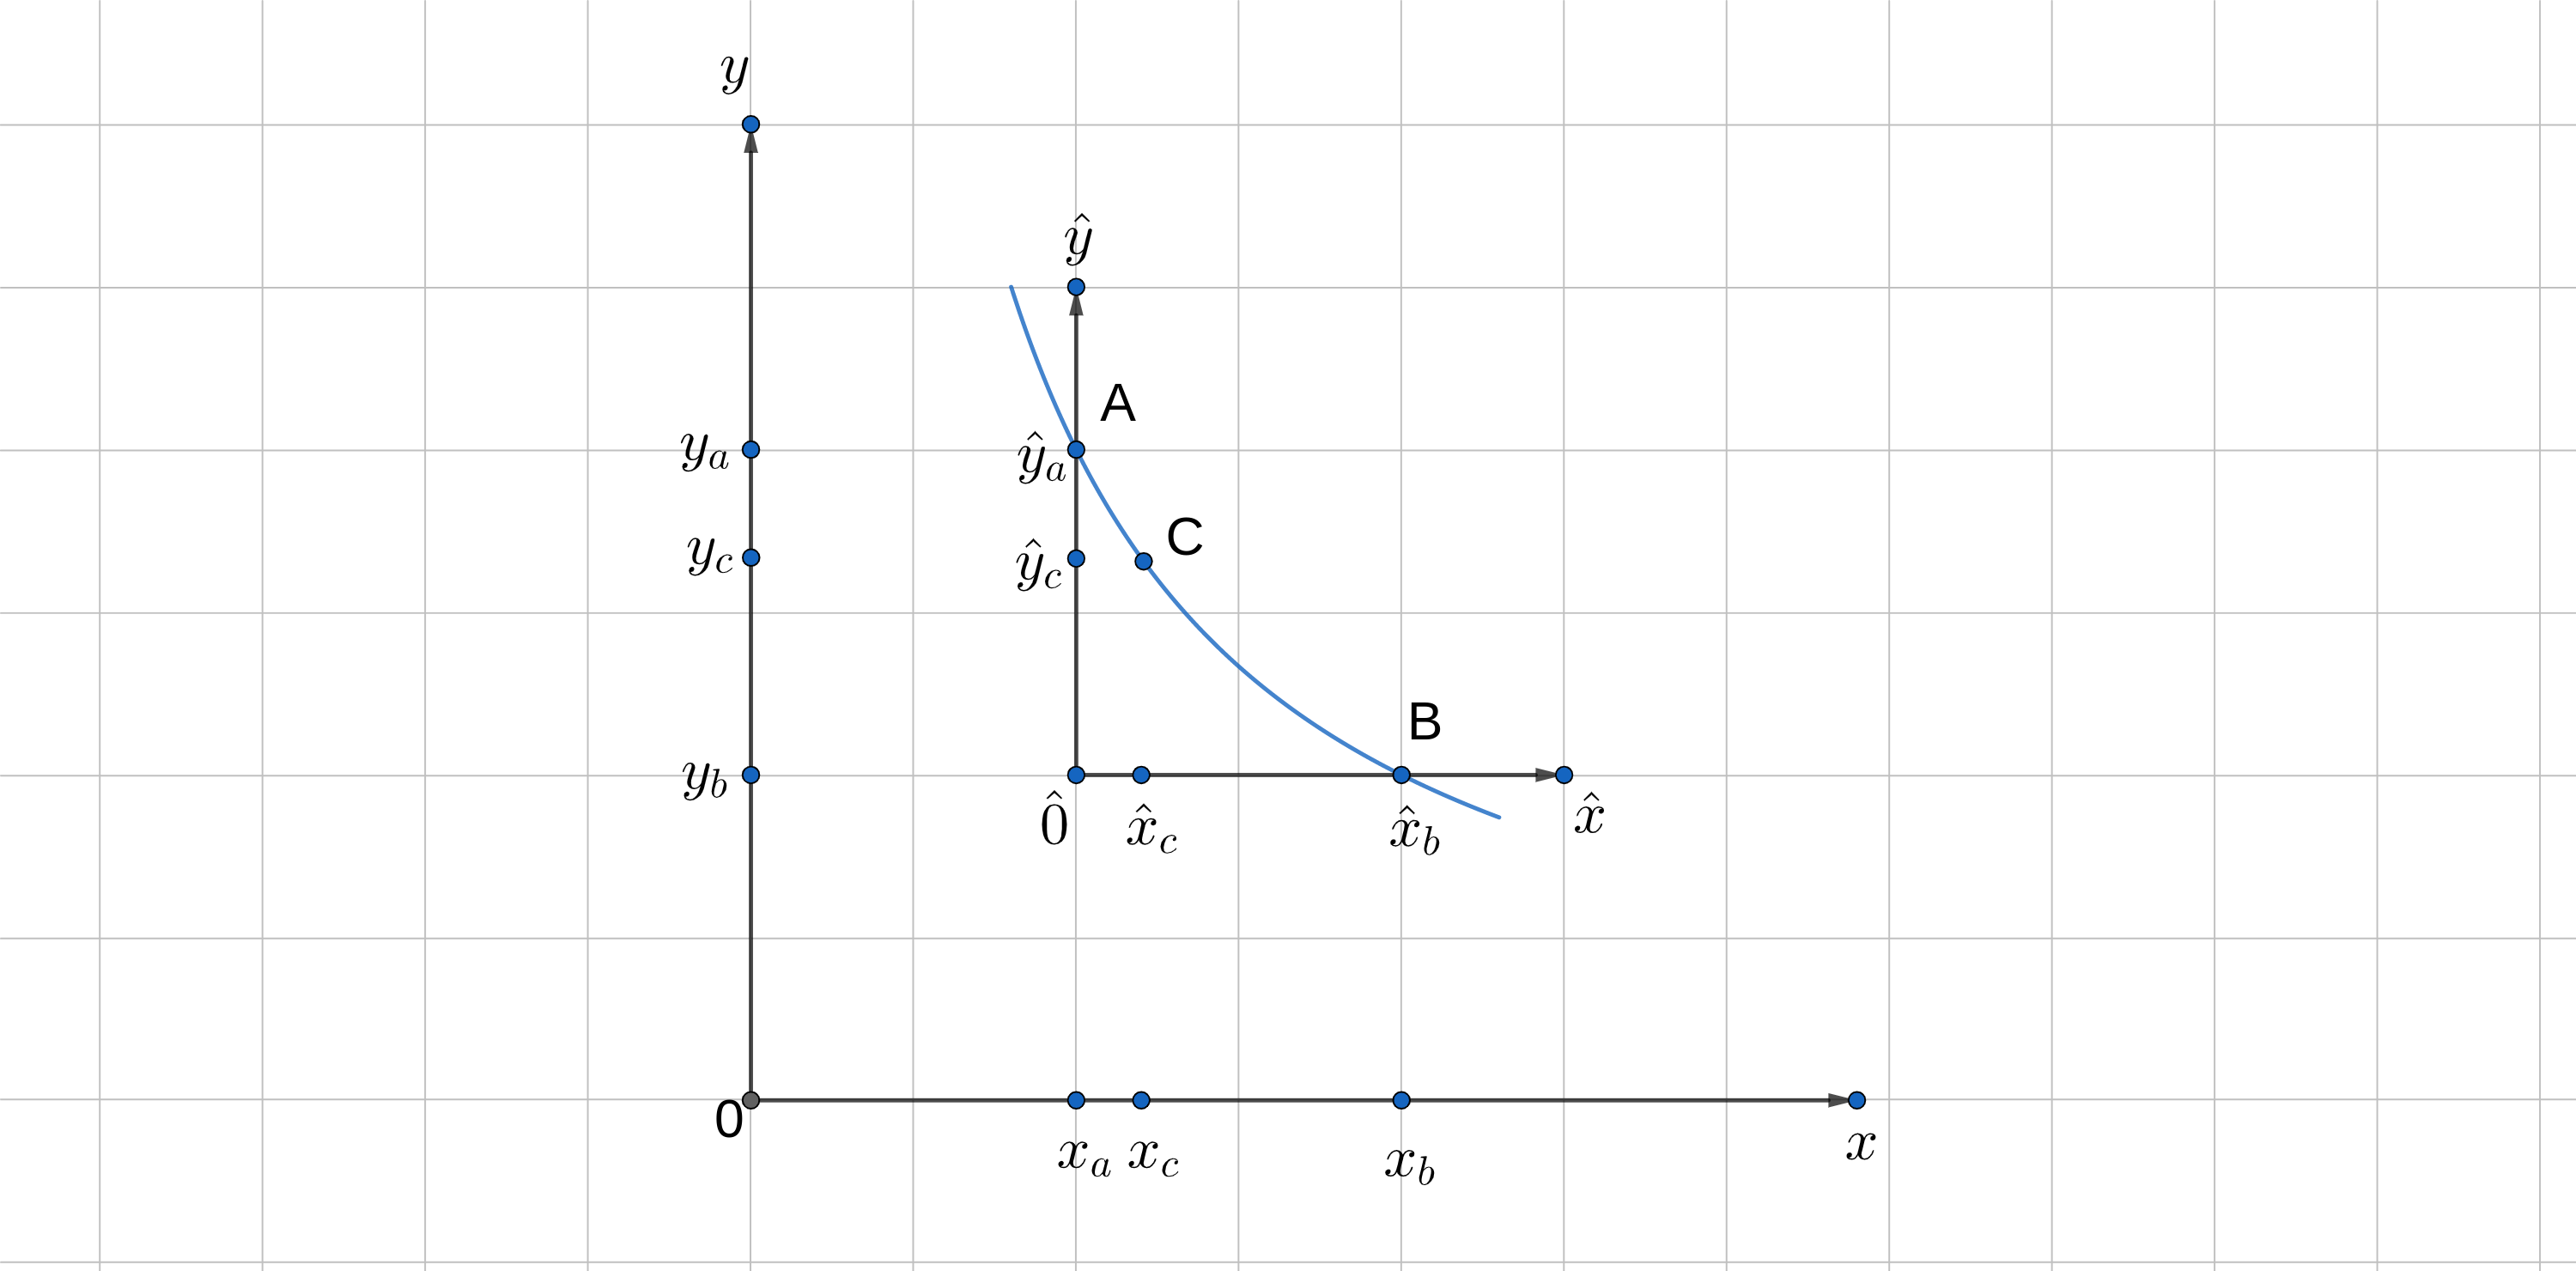
\includegraphics[scale=1.6]{uniswap_v3}
\centering
\caption{Real and virtual amounts axes.}
\end{figure}

Using Figure \ref{figure:uniswap_v3} as an example, given a price range defined by the points $A$ and $B$ in the $xy=k$ curve, the relationship between the real ($\hat{x}_c$) and virtual ($x_c$) amounts associated to a point $C$ between $A$ and $B$ can be stated as:

\begin{equation}
    \label{equation:virtual_amounts}
    \begin{split}
        x_c=\hat{x}_c + x_a \\
        y_c=\hat{y}_c + y_b \\
    \end{split}
\end{equation}


That distinction between virtual and real amounts enables Uniswap V3 to represent prices in a bounded price range $[p_a, p_b]$ with the same precision as Uniswap v2, however using less liquidity for this.
Again using Figure \ref{figure:uniswap_v3} as an example, in Uniswap V2, to represent the price in the point $C$, it would be necessary to have at least $x_c$ $tokens_x$ and at least $y_c$ $tokens_y$ available in the pool.
However, in Uniswap V3, if a liquidity provider decides to provide liquidity only in the price range $[p_a, p_b]$, then the price in the point $C$ requires only at least $\hat{x}_c$ and $\hat{y}_c$, in which $\hat{x}_c \leq x_c$ and $\hat{y}_c \leq y_c$.
Therefore, if liquidity providers choose price ranges wisely, capital efficiency is improved compared to Uniswap V2.
The downside is that, given a specific bounded Uniswap V3 position, not all prices can be represented, as can be noticed by analysing equation \ref{equation:virtual_amounts}, in which since virtual and real amounts are non-negative, it is not possible to represent virtual amounts $x_c$ smaller than $x_a$ nor $y_c$ smaller than $y_b$, meaning that possible prices lies only in $[p_a, p_b]$.

Different from Uniswap V2, Uniswap V3 doesn't directly track tokens amounts in the pool in its state, it tracks $L$ and $\sqrt{p}$ instead.
The reason behind this decision was convenience due to only one of those two values changing in an operation, i.e., $L$ changes when a liquidity provider adds/removes liquidity, and $\sqrt{p}$ changes when traders exchange tokens.
According to Uniswap V3 white paper this can also avoid some rounding issues that could arise due to tracking virtual amounts.
However, this complicates a little the understanding on how to calculate some properties related to a pool's state.

\subsection{Liquidity Providers Operations Invariance}

The invariance is the same as described in Section \ref{section:liquidity_providers_invariance}, however due to the way Uniswap V3 keeps states, a pool's state update in a operation is a little bit different.

First, it is possible to observe that current virtual amounts can be expressed as functions of $L$ and $\sqrt{p}$:

\begin{equation}
    \label{equation:x}
    \begin{split}
        p=\frac{y}{x}=\frac{k}{x^2}=\frac{L^2}{x^2} \\
        \Rightarrow x=\frac{L}{\sqrt{p}}
    \end{split}
\end{equation}

\begin{equation}
\label{equation:y}
    \begin{split}
        p=\frac{y}{x}=\frac{y^2}{k}=\frac{y^2}{L^2} \\
        \Rightarrow y=L\sqrt{p}
    \end{split}
\end{equation}

It is also possible to note that $L$ can be expressed in the following ways:

\begin{equation}
    \label{equation:l_x}
    \begin{split}
        x=\frac{L}{\sqrt{p}}=\hat{x} + x_a = \hat{x} + \frac{L}{\sqrt{p_a}} \\
        \Rightarrow L=\frac{\hat{x}\sqrt{p}\sqrt{p_a}}{\sqrt{p_a} - \sqrt{p}}
    \end{split}
\end{equation}

\begin{equation}
    \label{equation:l_y}
    \begin{split}
        y=L\sqrt{p}=\hat{y} + y_b = \hat{y} + L\sqrt{p_b} \\
        \Rightarrow L=\frac{\hat{y}}{\sqrt{p} - \sqrt{p_b}}
    \end{split}
\end{equation}

By \ref{equation:l_x} and \ref{equation:l_y}:

\begin{equation}
    \label{equation:real_x_y}
    \begin{split}
        \frac{\hat{x}\sqrt{p}\sqrt{p_a}}{\sqrt{p_a} - \sqrt{p}} = \frac{\hat{y}}{\sqrt{p} - \sqrt{p_b}} \\
        \Rightarrow \hat{y}=\frac{\hat{x}\sqrt{p}\sqrt{p_a}(\sqrt{p}-\sqrt{p_b})}{\sqrt{p_a}-\sqrt{p}}
    \end{split}
\end{equation}

Since $\sqrt{p}$, $\sqrt{p_a}$, $\sqrt{p_b}$ remains constant during a liquidity provider adding/removing liquidity operation, the following condition must be satisfied:

\begin{equation}
    \Delta_{\hat{y}}=\frac{\Delta_{\hat{x}}\sqrt{p}\sqrt{p_a}(\sqrt{p}-\sqrt{p_b})}{\sqrt{p_a}-\sqrt{p}}
\end{equation}

It is important to note that those equations only hold for $p \in [p_a, p_b]$, if this is not true, equations \ref{equation:virtual_amounts} are not valid.

Then, with those equations in hands it is possible to update $L$ after a liquidity provider operation.

\subsection{Handling Multiple Positions Simultaneously}

Uniswap V3 divides the price space in consecutive intervals called ticks.
When defining a price range, a liquidity provider actually defines a tick range, so not every price range is possible to be used as a pool's position.
At each time a pool is in a specific tick, and pool's price fluctuations due to trades can change the current pool's tick.
Once a pool leaves a tick and joins another the pool's liquidity is updated accordingly with the liquidity of the new tick.
A liquidity of a tick is the aggregated liquidity of all positions that include that tick.

\subsection{Zero-Sum Game}

Managing an Uniswap V3 position can be complex.
A liquidity provider must define which tick range to use, and also needs to be worried if this tick range will include the pool's price variations through time.
Both aspects will influence the amount of fees collected by the liquidity provider.
Then several protocols, such as Arrakis and Popsicle, arose to try to commoditize this management procedure, by providing an active Uniswap V3 position management service.

Today those active managers periodically update Uniswap V3 positions tick ranges in order to try to optimize fee collection to their users.
And they also bundle all its users in a single Uniswap V3 position, which can save some gas fees, since updating a single position for all users is cheaper than updating a single position for each user.

If we suppose a scenario in which the volume of trades is constant, which means that the amount of fees collected by trades is constant, if there is a single active manager that holds all the TVL in a V3 pool, then the fees earned by the liquidity providers will be the same as in a V2 pool, the tick range wouldn't matter in the amount of fees earned.
In the perspective of liquidity providers, who are interested in earning more fees, competition is interesting, it seems a zero-sum game, to some liquidity providers earn more fees others have to earn less.
Also, considering this, a liquidity provider doesn't want that other liquidity providers join the same active manager that he uses, since in this case there will be one less loser that he would benefit from.
But there is a trade-off here, due to more users in an active manager implicating in less gas cost overhead per user.
It seems that Uniswap V3 was not only a strategy to try to improve capital efficiency, to try to get more stable prices compared to V2, but also a strategy to create a gambling game, to keep liquidity providers interested in Uniswap, stimulating them to use different gambling strategies to try to earn more.

However it is possible to argue that concentrated liquidity increases the supply of liquidity providers, due to the gambling incentives, and also increases the demand for trades due to the improved price stability, which also increases the demand for liquidity providers, creating a feedback loop incentive.

\begin{thebibliography}{9}
\bibitem{uniswap_v3_whitepaper}
Hayden Adams, Noah Zinsmeister, Moody Salem, River Keefer, Dan Robinson. Uniswap v3 Core. March 2021.

\bibitem{uniswap_v2_whitepaper}
Hayden Adams, Noah Zinsmeister, Dan Robinson. Uniswap v2 Core. March 2020.

\bibitem{springer}
Mohan, V. Automated market makers and decentralized exchanges: a DeFi primer. Financ Innov 8, 20 (2022).

\end{thebibliography}

\end{document}
